%%%%%% Run at command line, run
%%%%%% xelatex grad-sample.tex 
%%%%%% for a few times to generate the output pdf file
\documentclass[12pt,oneside,openright,a4paper]{explo-english-project}

 \usepackage{polyglossia}
 \usepackage{graphicx,wrapfig,lipsum}
 \setdefaultlanguage{english}
 \setotherlanguage{thai}
\defaultfontfeatures{Mapping=tex-text,Scale=1.0,LetterSpace=0.0}
\setmainfont[Scale=1.0,LetterSpace=0,WordSpace=1.0,FakeStretch=1.0]{Times New Roman}
\emergencystretch=10pt
%\XeTeXlinebreaklocale "th_TH"	
%\XeTeXlinebreakskip = 0pt plus 1pt
%\setmathfont(Digits)[Scale=1.0,LetterSpace=0,FakeStretch=1.0]{Times New Roman}


%%% Title Page

% First line of title
\def\disstitleone{Project/Indep study title line 1}   
% Second line of title
\def\disstitletwo{Project/Indep title line 2 (optional)}   

% Members
\def\dissauthor{Ms. Pichyapa Khanapattanawong}
\def\dissauthortwo{Mr. Sakolkrit Pengkhum}
\def\dissauthorthree{Mr. Intouch Yuso}
\def\dissauthorfour{Ms. Ruedhaidham Soros}
\def\dissauthorfive{}

% The degree that you're persuing
\def\dissdegree{Bachelor of Engineering} 	% Name of the degree
\def\dissdegreeabrev{B.Eng} 				% Abbreviation of the degree
\def\dissyear{2021}                  		% Year of submission
\def\thaidissyear{2564}               		% Year of submission (B.E.)


%%% Project and independent study committee

\def\dissadvisor{Aye Thant May}  	% Main Teaching Assistant
% \def\disscommitteetwo{}  			% 3rd committee member (no-need)

\def\worktype{Project} 				% Project or Independent study
\def\disscredit{3}   				% 3 credits or 6 credits (no-need)

\def\fieldofstudy{Computer Engineering} 
\def\department{Computer Engineering} 
\def\faculty{Engineering}
 
\def\appendixnames{Appendix} %%% Appendices or Appendix

%%WWWWWWWWWWWWWWWWWWWWWWWWWWWWWWWWWWWWWWWWWWWWWWWWWWWWWWWWWWWWWWWWWWWWWWWWW%%

%%  ******** Do not modify from this part  ********
\def\thaidissadvisor{} % No-Need
%% Leave this empty if you have no co-advisor
\def\thaidisscoadvisor{} % No-Need
\def\thaidissdegree{วิศวกรรมศาสตรบัณฑิต}

% Change the line spacing here...
\linespread{1.15}

%%%%%%%%%%%%%%%%%%%%%%%%%%%%%%%%%%%%%%%%%%%%%%%%%%%%%%%%%%%%%%%%
% End of personal customization.  ******** Do not modify from this part  ********
% to \begin{document} unless you know what you are doing...
%%%%%%%%%%%%%%%%%%%%%%%%%%%%%%%%%%%%%%%%%%%%%%%%%%%%%%%%%%%%%%%%


%%%%%%%%%%%% Dissertation style %%%%%%%%%%%
%\linespread{1.6} % Double-spaced  
%%\oddsidemargin    0.5in
%%\evensidemargin   0.5in
%%%%%%%%%%%%%%%%%%%%%%%%%%%%%%%%%%%%%%%%%%%
%\renewcommand{\subfigtopskip}{10pt}
%\renewcommand{\subfigbottomskip}{-5pt} 
%\renewcommand{\subfigcapskip}{-6pt} %vertical space between caption
%                                    %and figure.
%\renewcommand{\subfigcapmargin}{0pt}

\renewcommand{\topfraction}{0.85}
\renewcommand{\textfraction}{0.1}

\newtheorem{theorem}{Theorem}
\newtheorem{lemma}{Lemma}
\newtheorem{corollary}{Corollary}

\def\QED{\mbox{\rule[0pt]{1.5ex}{1.5ex}}}
\def\proof{\noindent\hspace{2em}{\itshape Proof: }}
\def\endproof{\hspace*{\fill}~\QED\par\endtrivlist\unskip}
%\newenvironment{proof}{{\sc Proof:}}{~\hfill \blacksquare}
%% The hyperref package redefines the \appendix. This one 
%% is from the dissertation.cls
%\def\appendix#1{\iffirstappendix \appendixcover \firstappendixfalse \fi \chapter{#1}}
%\renewcommand{\arraystretch}{0.8}
%%%%%%%%%%%%%%%%%%%%%%%%%%%%%%%%%%%%%%%%%%%%%%%%%%%%%%%%%%%%%%%%
%%%%%%%%%%%%%%%%%%%%%%%%%%%%%%%%%%%%%%%%%%%%%%%%%%%%%%%%%%%%%%%%


\begin{document}
\pdfstringdefDisableCommands{%
\let\MakeUppercase\relax
}
\begin{center}
  
\includegraphics[width=2.8cm]{./assets/unilogo.jpg}
\end{center}
\vspace*{-1cm}

\maketitlepage
%\makesignaturepage 

% abstract page
%%WWWWWWWWWWWWWWWWWWWWWWWWWWWWWWWWWWWWWWWWWWWWWWWWWWWWWWWWWWWWWWWWWWWWWWWWW%%
%%%%%%%%%%%%%%%%%%%%%%%%%%%%%%%%%%%%%%%%%%%%%%%%%%%%%%%%%%%%%%
%%%%%%%%%%%%%%%%%%%%%%         English abstract         %%%%%%%%%%%%%%%%%%%%%%%
%%%%%%%%%%%%%%%%%%%%%%%%%%%%%%%%%%%%%%%%%%%%%%%%%%%%%%%%%%%%%%
%%WWWWWWWWWWWWWWWWWWWWWWWWWWWWWWWWWWWWWWWWWWWWWWWWWWWWWWWWWWWWWWWWWWWWWWWWW%%
\abstract

In a multihop ad hoc network, the interference among nodes is
  reduced to maximize the throughput by using a smallest transmission
  range that still preserve the network connectivity. However, most
  existing works on transmission range control focus on the
  connectivity but lack of results on the throughput performance. This
  paper analyzes the per-node saturated throughput of an IEEE 802.11b
  multihop ad hoc network with a uniform transmission range. Compared
  to simulation, our model can accurately predict the per-node
  throughput.  The results show that the maximum achievable per-node
  throughput can be as low as 11\% of the channel capacity in a normal
  set of $\alpha$ operating parameters independent of node density. However, if
  the network connectivity is considered, the obtainable throughput
  will reduce by as many as 43\% of the maximum throughput. YOOO

\begin{flushleft}
\begin{tabular*}{\textwidth}{@{}lp{0.8\textwidth}}
\textbf{Keywords}: & Multihop ad hoc networks / Topology control / Single-Hop Throughput
\end{tabular*}
\end{flushleft}
\endabstract

% acknowledgements
% Acknowledgements

\preface
Acknowledge your advisors and thanks your friends here..

% table of contents (autogen)
\tableofcontents   

% list of tables (autogen)
\listoftables

% list of figures (autogen)
\listoffigures                      

% list of symbols
% List of symbols 

\listofsymbols
\begin{flushleft}
\begin{tabular}{@{}p{0.07\textwidth}p{0.7\textwidth}p{0.1\textwidth}}
\textbf{SYMBOL}  & & \textbf{UNIT} \\[0.2cm]
$\alpha$ & Test variable\hfill & m$^2$ \\
$\lambda$ & Interarival rate\hfill &  jobs/second\\
$\mu$ & Service rate\hfill & jobs/second\\
\end{tabular}
\end{flushleft}

% list of vocabulary
\include{./chapters/preface/ListVocabs}

%\setlength{\parskip}{1.2mm}



%%%%% Main Body %%%%%

%%% Chapter 1 - Introduction

\chapter{Introduction}

% Sections in introduction

\section{Background} 
% put the content here

This is the background of the project.

% example for pictures
% \begin{figure}[!h]
% \centering
% 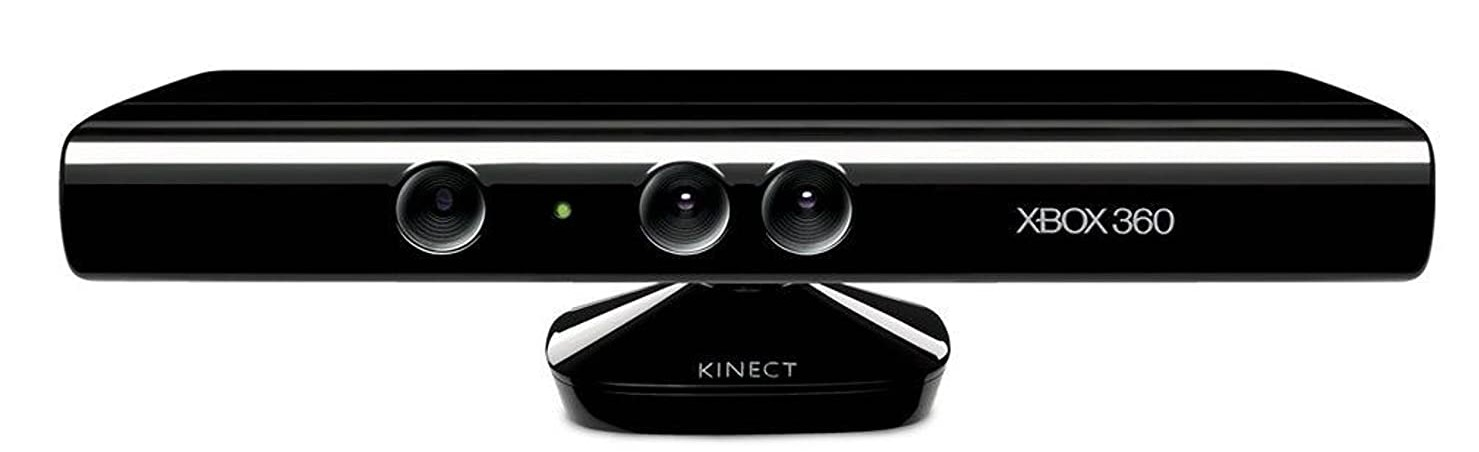
\includegraphics[width=90mm]{X11.jpg}
% \caption{This is the figure Kinect Xbox}\label{fig:x1}
% \end{figure}


\section{Motivations}
% Put the content here
This is our motivations.

% Example for unordered list
\begin{itemize}
\item   What are the problems you are addressing? 
\item  Why they are important?
\item  What are the limitations of existing approaches? 
\end{itemize}
You may combine this section with the background section.

\section{Problem Statements}
% Put content here
This is our problem statement.

\section{Objectives}
% Put content here
This is our objectives.

\section{Scope of Work}
% Put content here
This is our scope.

\section{Project Schedule}
% Put content here

This is our schedule


%%% Chapter 2 - Background Theory and Related work

\chapter{Background Theory and Related Work}

% Create sections and input content files related to background here
\section{Games as an Education Medium}
% Game as an Education Medium
\medskip
\subsection{Games Popularity Around the World}
\url{https://financesonline.com/number-of-gamers-worldwide/}
comprises of statistics, demographics, and predictions related to games and gamers 
both worldwide and by region. [Nestor Gilbert]

According to NewZoo Research (2020), there were 2.69 billion gamers in the world by the end of 2020. From the statistics, it is to be expected that the number of gamers will continue to rise, expecting to reach 2.95 billion gamers worldwide in 2022.

% Active gamers
\begin{figure}[!h]\centering
\setlength{\fboxrule}{0.2mm} % can define this in the preamble
\setlength{\fboxsep}{0.5mm}
\fbox{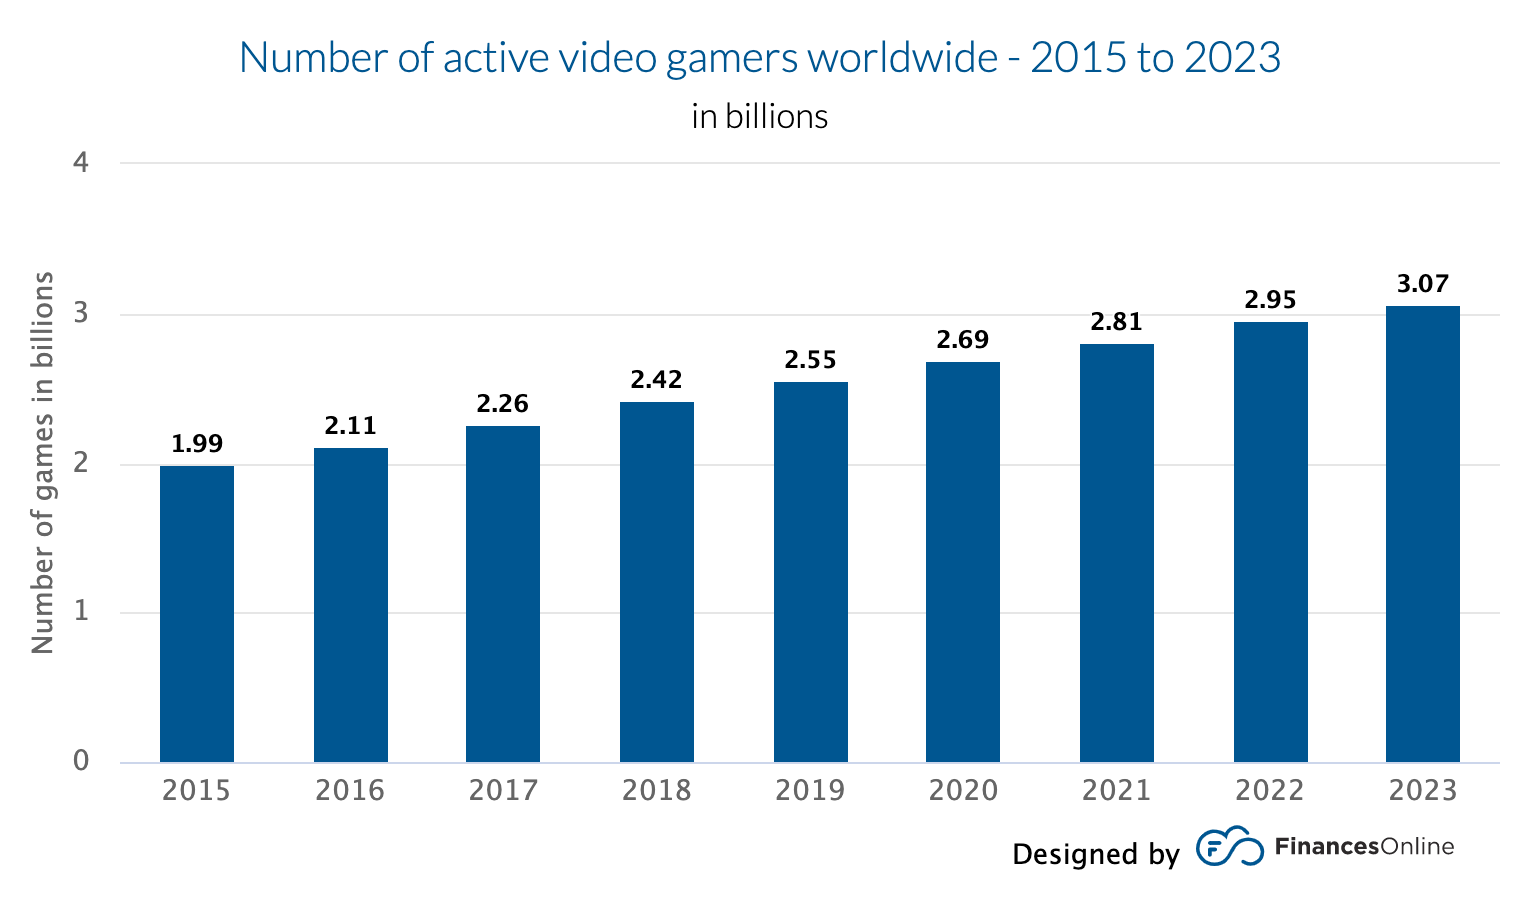
\includegraphics[width=8cm]{./assets/graph_active_gamers.png}}
\caption{Numbers of active gamers worldwide}\label{fig:model2}
\end{figure}

Looking further into the age group of gamers. Limelight's research(2020) suggests that every gamers ranging from age 18 - 64 years old spend at least 4.7 hours per week playing games, with the highest hours of 7.48 in 18 - 25 age group.

% Hours
\begin{figure}[!h]\centering
\setlength{\fboxrule}{0.2mm} % can define this in the preamble
\setlength{\fboxsep}{0.5mm}
\fbox{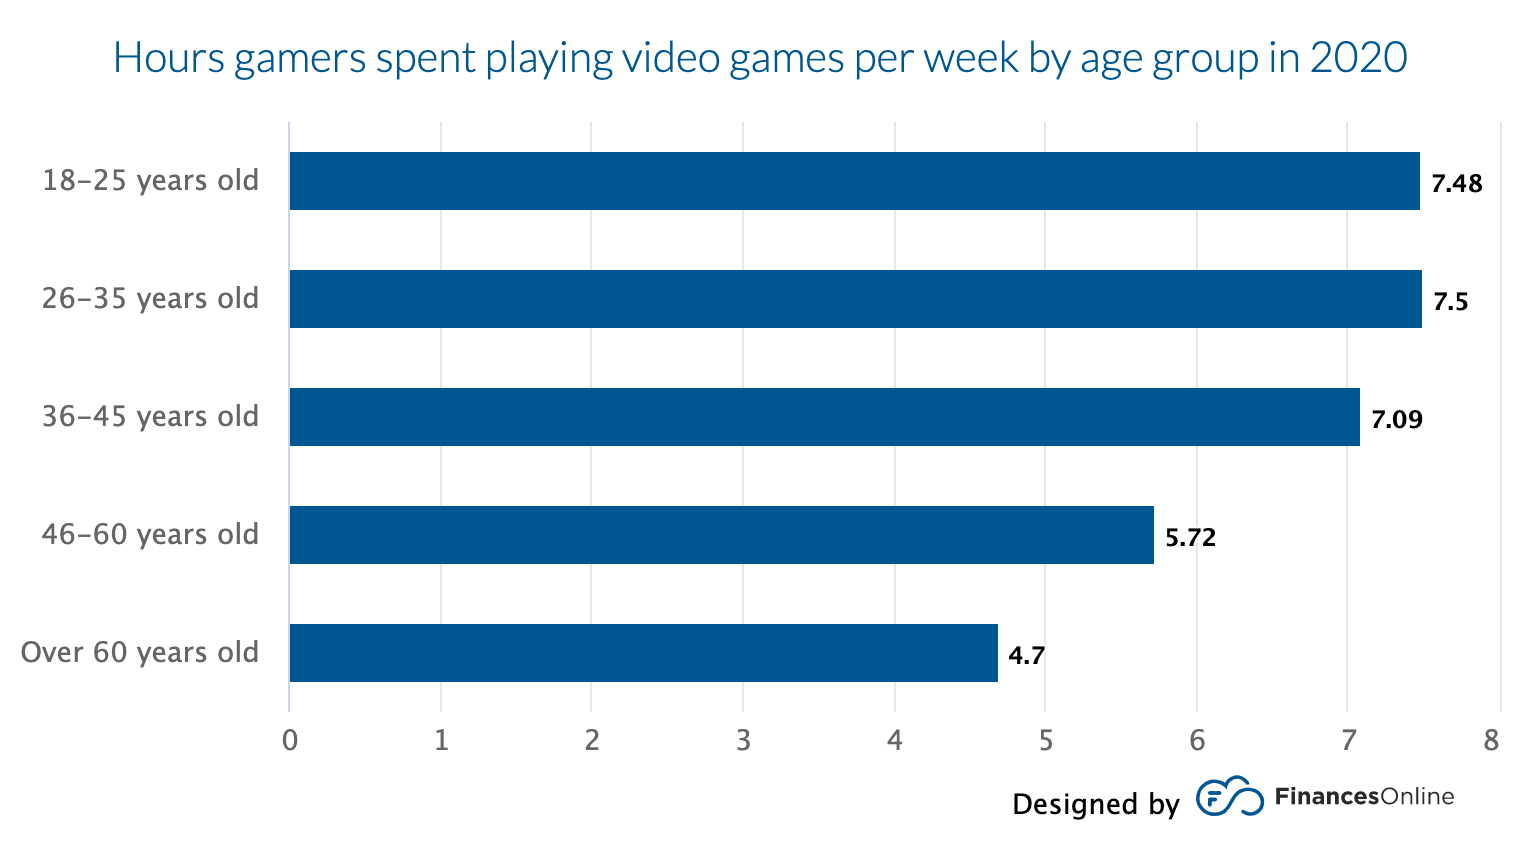
\includegraphics[width=8cm]{./assets/graph_gaming_hours.png}}
\caption{Average gaming hours per week by age group}\label{fig:model2}
\end{figure}

Game is currently one of the largest markets. Its revenues for 2020 reached over 159.3 billion US Dollars with almost half of market earnings generated by the Asia Pacific region. Evidently, game is a useful tool that can reach out to a broad range of people, which is why the demand for educational games are increasing especially during the pandemic where classes are taught online.\\[2cm]


\subsection{Application of Educational Games and its effectiveness}
\url{https://research.com/education/interactive-learning-statistics#5} provides statistics, demographics, and predictions related to educational games and active learning methods. [Imed Bouchrika]
Interactive learning is a learning method that supports the communications and interactions between educators and students. One of the effective ways to achieve active learning is through games. Juraschka (2019) showed that 74\% of teachers used game-based learning to enhance their lessons. This also applies in other settings other than the classroom as well, such as workplace and companies, which evidently increased the compound annual growth rate by half according to Ibáñez research (2018)\\

These research paper suggests the effects that educational games have on students.\\
\url{https://www.frontiersin.org/articles/10.3389/feduc.2021.623793/full} focused on educational games and learning effectiveness on college students [Siu Yin Cheung, Kai Yin Ng]\\
\url{https://www.sciencedirect.com/science/article/pii/S1875389212015933} analyzes the relationship between educational games and mathematics and logic. [Jing Li, Sujuan Ma, Linqing Ma]\\
\url{https://educationaltechnologyjournal.springeropen.com/articles/10.1186/s41239-017-0062-1} explores the effects of games and simulations on higher educatio.n [Dimitrios Vlachopoulos, Agoritsa Makri]\\
\url{https://www.researchgate.net/publication/233279860_Motivating_Children_to_Learn_Effectively_Exploring_the_Value_of_Intrinsic_Integration_in_Educational_Games}
suggests that motivations are the important aspect of using games as a educational tool. [Jacob Habgood, Shaaron Ainsworth]\\

Evidently, games are one of the effective methods to conduct interactive class and active learning for students. It can provide motivation and stimuli for students, and can effectively help them understand the concept they're trying to learn more deeply and entertainingly.


\subsection{Educational Game Specifications}
\url{https://www.researchgate.net/publication/267034149_Educational_Games_for_Teaching_Computer_Programming} page 3, in the topic educational games requirement specification suggests what aspects should be included in an effective educational game.\\
It is suggested that it should include two main aspects which are\\
1. Cognitive axis: Information intended to be received by the students should begin from the first category in the Bloom's taxonomy. 
\vspace{-5mm}
\paragraph{Bloom's Taxonomy} 

%------------------------------------------
\begin{wrapfigure}{lh}{7.5cm}
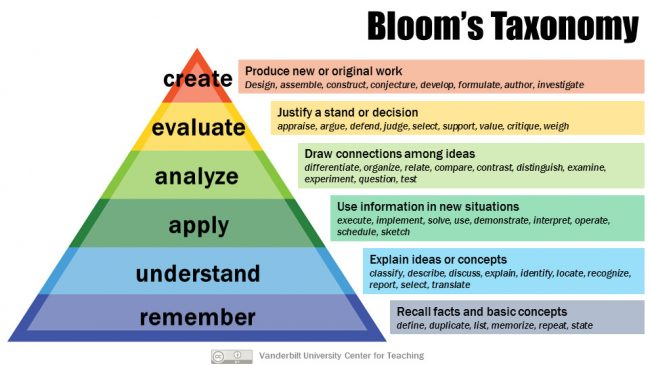
\includegraphics[width=7.5cm]{./assets/bloom.jpeg}
\end{wrapfigure} 
This is the structure of Bloom's Taxonomy, a taxonomy for teaching, learning, and assessment. It'll help us plan and design effective questions and puzzle for our game. Besides, we can ensure that our game lessons align with the objectives of teaching the fundamental of AI.
\\
\par
2. Emotional axis: Enable students to handle given situations through emotions, and using it to motivate students to solve and learn faster. So, they can experience the accomplishments when they get to the end of the story.

\section{Importance of Artificial Intelligence}
\medskip
\subsection{Artificial Intelligence from Global Perspective}
\url{https://mitsloan.mit.edu/ideas-made-to-matter/new-report-details-growing-global-interest-artificial-intelligence}, a report from 2018, shows that interest in AI from a global level has been increasing rapidly in the past few decades.\\
Presently in 2021, the interest is still growing. Even more so when there are so many new technologies emerging that will require the power of AI to solve. Research focusing on AI has drastically increased. AI is applied to many aspect of our lives and work such as engineering, society, medications, and so on. So, it's crucial that everyone, interested in developing AI or not, knows the fundamental of AI as it will have a critical role in our daily lives in the near future.

\subsection{Artificial Intelligence in Thailand}
\url{https://thaiembdc.org/2021/04/28/ai-and-robotics-growing-rapidly-in-thailand/} \\ suggests the trend of AI in Thailand and shows related statistics.\\
Similar to the global level, AI in Thailand is also growing at a rapid rate. We have the foundation ready for AI and automation industry. So, it's predicted that AI trend will grow in the future to support the country's economic, industry, and increase productivity.

\subsection{Existing Learning Source about AI}
\paragraph{University Curriculum about AI in Thailand}
In some universities, AI education exists in the form of an extra credit that students can choose to apply.\\
\url{https://www.admissionpremium.com/content/5909} shows the courses that major in AI engineering. There are only 2 public universities that currently have the AI engineering department which are King Mongkut's Institute of Technology Ladkrabang and Chulalongkorn University. Others are private universities which are considerably more costly than private universities.

\subsection{Online AI courses and Educational Programming Games}
There are a lot of online courses available for learning AI such as Udemy, coursera, edX, and so on. There are also educational games for learning coding fundamentals such as Code Combat, Minecraft: Hour of Code, Scratch, and lots more. But when it comes to educational games for AI, there are quite a few. Some are focused on competitive AI coding which is not friendly for beginner. \\
\url{https://studio.code.org/s/oceans/} This is an interesting example of games that teach the concept of AI. It has a great design and concepts, cute gameplay, and good for learning the basic of AI and image recognition. 
\vspace{-5mm}
\paragraph{Educational Games and Programming} ~\\
\url{https://www.researchgate.net/publication/305084679_Learning_Programming_through_Games_and_Contests_Overview_Characterisation_and_Discussion}
reviews some good platform to learn programming. \\[5cm]
\url{https://www.researchgate.net/publication/267034149_Educational_Games_for_Teaching_Computer_Programming} discusses about important characteristics of educational coding games. Additionally, it goes over some educational programming games and their uniqueness as well. \\
\url{https://files.eric.ed.gov/fulltext/EJ1233506.pdf} explores the effectiveness of using games to teach programming concepts and problem solving skills. The game used in this research is PROSOLVE. \\
These researches provide us with great resource of how our game should be in order to be effective for the players to learn while playing. It also proves that games are useful for learning programming concepts as well.

\section{Development Tools}
\medskip
\subsection{Miro}
\url{https://miro.com/app/dashboard/} is an online whiteboard and visual collaboration platform. This is what we use to organize our ideas, storyboard, and role as it is a good tool for working and brainstorming online. 
\subsection{Notion}
\url{https://www.notion.so/} is an application that provides components such as notes and databases. Providing lots of tools and blocks, notion can help users their own systems for note taking and data management. We use it to store our information and meeting notes. 
\subsection{Microsoft Planner}
\url{https://tasks.office.com/mail.kmutt.ac.th/en-US/Home/Planner/} is a project management tool that will help users manage their tasks and projects. We use it to distribute tasks and our project timeline. 
\subsection{Fire Alpaca and Clip Studio Paint}
\url{https://firealpaca.com/} and \url{https://www.clipstudio.net/en/} are tools for creating computer graphics. We use these to create pixel art for maps and sprites in our games.
\subsection{Garage Band}
\url{https://www.apple.com/mac/garageband/} is a line of digital audio workstations for macOS, iPadOS, and iOS devices that allows users to create music or podcasts. We use this tool to create soundtracks and background music for our games.
\subsection{GitHub}
\url{https://github.com/} is a provider of Internet hosting for software development and version control using Git. We use it to share our code, work collaboratively online, and manage the version control for our game.
\subsection{Godot Engine}
\url{https://godotengine.org/} is a cross-platform, free and open-source game engine released under the MIT license. We use this tool to develop our game because it is well documented, beginner friendly, and appropriate for our game.
% 1. Games as education medium
	% 3. Educational Games Specification
% 2. Importance of AI
% 3. Educational Programming games


% Algorithms, related work, development tools

% Example table
% \begin{table}[!h]
% \caption{test table method1}\label{tbl:method1}
% \begin{tabular}{c|c|l|rr} \hline\hline
% Center & Center & left aligned & Right & Right aligned \\ \hline\hline
% Center & Center & left aligned & Right & Right aligned \\ \hline
% \end{tabular}
% \end{table}

% \subsection{Algorithm I}

% Example picture
% \begin{figure}[!h]\centering
% \setlength{\fboxrule}{0.2mm} % can define this in the preamble
% \setlength{\fboxsep}{1cm}
% \fbox{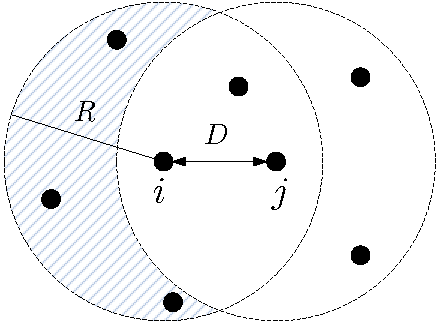
\includegraphics[width=5cm]{./model2.pdf}}
% \caption{The network model}\label{fig:model2}
% \end{figure}


%%% Chapter 3 - Proposed Work

\chapter{Proposed Work}

% Sections in Proposed Work

\section{Graphic Designs}
% put content here
% Character design, map design
% /subsection{}
This is graphic design

\section{Puzzle Design}
% Put content here
% Puzzle questions, puzzle mechanics

This is puzzle design

\section{UXUI Design}
% Put content here
% UXUI Design, User interface,...

This is uxui design

\section{Game Story}
% Put content here
% Game story

This is the game story

\section{Music Design}
% Put content here
% Music Design

This is music design

\section{Dialogue and Interaction}
% Put content here
% dialogue, npc interaction, effects to ending, stat

This is the interactions


%% Chapter 4 - Implementation and results
% implementation / experimental results

\chapter{Implementation Results}

% put content here

% if you want sections
% \section{}
% \input{./chapters/implement/...}


%%% Chapter 5 - Conclusion

\chapter{Conclusions}

\section{Problems and Solutions}
% Problems and solutions

State problems and how you fixed them

\section{Future Works}
% Future Work
What could be done in the future to make your projects better.


%%%%% End of Main body %%%%%


%%% Bibliography
%%%% Comment this in your report to show only references you have
%%%% cited. Otherwise, all the references below will be shown.
%\nocite{*}
%% Use the kmutt.bst for bibtex bibliography style 
%% You must have cpe.bib and string.bib in your current directory.
%% You may go to file .bbl to manually edit the bib items.

\makeatletter
\g@addto@macro{\UrlBreaks}{\UrlOrds}
\makeatother

\bibliographystyle{kmutt}
\bibliography{string,cpe}


%%% Appendices

\appendix{First appendix title}
\noindent{\large\bf Put appropriate topic here} 

% Put content here		% First Appendix
\appendix{Second appendix title}
\noindent{\large\bf Put appropriate topic here} \\

Next, we show how $\mathrm{Var}\{X_n\}$ can be determined.  Let
$C_{\lambda}(l)$ be the autocovariance function of $\lambda_n$.  The
MVA technique basically approximates the input process $\lambda_n$
with a Gaussian process, which allows $\mathrm{Var}\{X_n\}$ to be
represented by the autocovariance function.  In particular, the
variance of $X_n$ can be expressed in terms of $C_{\lambda}(l)$ as
\begin{equation}
  \mathrm{Var}\{X_n\} = nC_{\lambda}(0) + 2\sum_{l=1}^{n-1} (n-l)C_{\lambda}(l)
\end{equation} 

\noindent{\large\bf Add more topic as you need} \\

Therefore, $C_{\lambda}(l)$ must be known in the MVA technique, either
by assuming specific traffic models or by off-line analysis in case of
traces.  In most practical situations, $C_{\lambda}(l)$ will not be
known in advance, and an on-line measurement algorithm developed
in~\cite{eun01} is required to jointly determine both $n^\ast$ and
$m_x$. For fGn traffic, $\mathrm{Var}\{X_n\}$ is equal to $\sigma^2
n^{2H}$, where $\sigma^2 = \mathrm{Var}\{\lambda_n\}$, and we can find
the $n^\ast$ that minimizes (\ref{eq:mx}) directly. Although $\lambda$
can be easily measured, it is not the case for $\sigma^2$ and $H$.
Consequently, the MVA technique suffers from the need of prior
knowledge traffic parameters. 		% Second Appendix

\end{document}
